\chapter{Sending and Receiving Interactions}
\label{sec:hla-inter}

This section illustrates how to use \TrickHLA\ to
send and receive HLA interactions.
The example simulations are similar to the publisher and
subscriber simulations discussed earlier, but in this case,
the subscriber's sine parameters have been initialized with
a zero-value amplitude.
Thus, the subscriber's state is initially constant,
$x(t)=0$, $\dot{x}(t)=0$.
However, at a certain point in the simulation,
the publisher sends its sine parameters
(in particular, a non-zero amplitude)
to the subscriber in an interaction.
Once the subscriber receives these values and updates the appropriate
Trick variables, $x(t)$ and $\dot{x}(t)$ assume their expected sine wave
shapes.\footnote{
  No state data are exchanged in this interaction, only the
  \simplesine parameters, $A$, $\phi$ and $\omega$.
  The calculation of the state on the subscriber side is only used as a
  way to graphically illustrate the arrival of the interaction from the
  publisher.
}

% -----------------------------------------------------------------------
\section{What is an interaction handler?}
% -------------------------------
\subsection{The class {\tt TrickHLAInteractionHandler}}

\TrickHLA\ defines a C++ class which may be subclassed by
simulation developers in order to send or receive interactions.
The class header is shown below.
It defines {\em send} and {\em receive} methods which may be called
by simulation developers,
avoiding the need to directly use the {\tt TrickHLAInteraction} class,
which is fairly complex.

There are actually two send methods.
The one with no arguments, sends the interaction to the receiver,
where it is delivered in the order interactions arrive off the network.
The send method with a single timetag argument sends the interaction
to receivers where it is delivered in time stamp order.
The timetag argument must be a simulation timetag plus some lookahead
interval.
These send methods are sufficient unto themselves and do not need to
be overridden in a subclass.  Indeed they are not virtual methods.

The receive method is virtual.
The \TrickHLA\ infrastructure will automatically invoke a subclass's
corresponding version of the method when interactions arrive from remote
senders.

The protected {\tt interaction} field may be ignored.
The \TrickHLA\ infrastructure automatically takes care of creating
interactions according to the declarations encountered in the input file.

\begin{lstlisting}[caption={The {\tt TrickHLAInteractionHandler} class},label={list:trickhla-interaction-handler}]
class TrickHLAInteraction;
#include "TrickHLA/include/TrickHLAInteraction.hh"

class TrickHLAInteractionHandler
{
   friend class InputProcessor;
   friend void init_attrTrickHLAInteractionHandler();

  public:
   TrickHLAInteractionHandler();
   virtual ~TrickHLAInteractionHandler();

   virtual void initialize_callback( TrickHLAInteraction * inter );

   bool send_interaction(); // Receive Order
   bool send_interaction( double send_time ); // Timestamp Order

   TrickHLADoubleInterval get_fed_lookahead();
   TrickHLADoubleTime     get_granted_fed_time();
   
   virtual void receive_interaction();

  protected:
   TrickHLAInteraction * interaction;
};
\end{lstlisting}

% -------------------------------
\subsection{Interaction handling in \simplesine}

The class header for the \simplesine interaction handler is shown below.


\begin{lstlisting}[caption={{\tt simplesine\_InteractionHandler} header file},label={list:simplesine-interaction-handler-header}]
#include "TrickHLA/include/TrickHLAInteractionHandler.hh"

class simplesine_InteractionHandler : public TrickHLAInteractionHandler
{
  friend class InputProcessor;
  friend void init_attrsimplesine_InteractionHandler();

  public:
    simplesine_InteractionHandler();
    virtual ~simplesine_InteractionHandler();

    void send_sine_interaction( double send_time );
    virtual void receive_interaction();

  protected:
    double lookahead_time;
};
\end{lstlisting}

And the methods are shown below.
The {\tt send\_sine\_interaction()} method is just a wrapper around the
parent class's {\tt send\_interaction()} method.

And the {\tt receive\_interaction()} method, just invokes the Trick
output function, {\tt send\_hs()} to indicate that an interaction arrived;
by the time the receive method is invoked,
the data from the incoming interaction have already been stored in the
Trick variable that is associated with the interaction in the input
file.  (See below.)
So there is nothing much to do in the implementation of the receive method.

\begin{lstlisting}[caption={{\tt simplesine\_InteractionHandler} methods},label={list:simplesine-interaction-handler-methods}]
/********************************* TRICK HEADER *******************************
PURPOSE: (Send/receive HLA interactions.)
*******************************************************************************/

#include <stdlib.h>
#include <string>
#include "../include/simplesine_InteractionHandler.hh"

using namespace std;

/* ----------------------------------------------------------------------------
PURPOSE: (Default constructor)
------------------------------------------------------------------------------*/
simplesine_InteractionHandler::simplesine_InteractionHandler() // RETURN: -- None.
: lookahead_time(0.0)
{ }


/* ----------------------------------------------------------------------------
PURPOSE: (Destructor.)
------------------------------------------------------------------------------*/
simplesine_InteractionHandler::~simplesine_InteractionHandler() // RETURN: -- None.
{ }


/* ----------------------------------------------------------------------------
PURPOSE: (Send this handler's HLA interaction.  A pointer to the interaction
  is stored in this class -- defined in the protected <interaction> field
  in the parent class.  The TrickHLA infrastructure takes care of setting
  that pointer when it sees interactions declared in the Trick input file.)
------------------------------------------------------------------------------*/
void simplesine_InteractionHandler::send_sine_interaction( // RETURN: -- None.
   double send_time )        // IN: s HLA time to send the interaction.
{
   const char* FOM_name = (const char*)this->interaction->get_FOM_name();
   bool interaction_was_sent = false;
   double timetag = send_time + lookahead_time;

   bool was_sent = this->TrickHLAInteractionHandler::send_interaction( timetag );

   if( was_sent ) {
      const char* msg = string("sent interaction: ").append(FOM_name).c_str();
      send_hs( stdout, (char*)msg );
   } else {
      const char* msg = string("error sending interaction: ").append(FOM_name).c_str();
      send_hs( stderr, (char*)msg );
   }
}


/* ----------------------------------------------------------------------------
PURPOSE: (Handle an incoming interaction.)
------------------------------------------------------------------------------*/
void simplesine_InteractionHandler::receive_interaction() // RETURN: -- None.
{
   const char* FOM_name = (const char*)this->interaction->get_FOM_name();
   const char* msg = string("Received interaction: ").append(FOM_name).c_str();

   send_hs( stdout, (char*)msg );
}
\end{lstlisting}

% -----------------------------------------------------------------------
\section{\tt SIM\_simplesine\_hla\_sendInt}

This simulation is based on the publisher simulation,
{\tt SIM\_simplesine\_hla\_pub} even though it does no real publishing.
Instead, it just sends an interaction once during the simulation.
The interaction handler {\em send} method is invoked at a specified
time during the simulation, using the Trick {\tt CALL} directive.\footnote{
  More sophisticated simulations might call the method
  directly from simulation-specific code.
  We do not do that here.
}
To do this, you must do two things to the \sdefine file.

\begin{itemize}
\item{
  Define an instance of the interaction handler, and
}
\item{
  Specify a 0-frequency job for the {\em send} method.\footnote{
    0-frequency jobs are a common way to force Trick to generate
    code for the job even though it is not actually part of the
    periodically scheduled jobs.
    In this case,
    the send method is not invoked from a regularly scheduled job,
    but from a single invocation of it as specified in the input file.
    If we did not specify a 0-frequency job like this, Trick would
    not compile the code for the job, and we would get a runtime error.
  }
}
\end{itemize}

Thus, the {\tt publisher} sim object for this simulation has two
lines that do not appear in the plain publisher:

\begin{lstlisting}[numbers=none,caption={Sending interaction handler \sdefine changes},label={list:sending-interaction-handler-sdefine-changed}]
  sim_object {
    ...
    simplesine: simplesine_InteractionHandler interaction_handler;
    ...
    (0.0, scheduled) simplesine:
      publisher.interaction_handler.send_sine_interaction(
        In double time = sys.exec.out.time );
    ...
} publisher;
\end{lstlisting}

% -----------------------------------------------------------------------
\section{Sender input}

The sender's input file is based on the plain publisher's input file.
They differ in the following ways.
\begin{itemize}
\item{
  The federate name is {\em sender} instead of {\em publisher},
  and it waits for the {\em receiver} federate instead of {\em subscriber},
}
\item{
  since this simulation does not actually publish anything,
  there are no objects and attributes defined,
}
\item{
  the interaction handler lookahead time is specified,
}
\item{
  the interaction and parameters to be sent are specified, and
}
\item{
  there is a {\tt CALL} directive invoking the interaction handler
  method, {\tt send\_sine\_interaction()}.
}
\end{itemize}

The complete input file is listed in
Appendix~\ref{sec:send-receive-inputs}
on page~\pageref{sec:complete-sender-input}.

% -----------------------------------------------------------------------
\section{\tt SIM\_simplesine\_hla\_receiveInt}

This simulation is based on the plain subscriber simulation,
{\tt SIM\_simplesine\_hla\_sub} even though it does no real subscribing.
Instead, it just waits for an interaction to arrive.
The \TrickHLA\ infrastructure automatically handles incoming interactions
and assigns the associated parameter values to Trick variables
as specified in the input file.  (See next section.)
There are no explicit jobs to schedule in the \sdefine file,
and there are no jobs to {\tt CALL} from the input file, either.

To do this, all you need to do is declare an interaction handler
in the {\tt subscriber} sim object.\footnote{
  Unlike the case of sending interactions,
  receiving interactions requires no jobs be executed by Trick.
  Consequently, in this case (unlike the interaction sender),
  there is no need to declare a zero-frequency job in the \sdefine file.
}

The \sdefine for the receiver is virtually identical with that of the
plain subscriber with the following exceptions.

\begin{itemize}
\item{
A interaction handler variable is defined:
\begin{verbatim}
 simplesine: simplesine_InteractionHandler interaction_handler;
\end{verbatim}
}
\item{
The numerical integration of the the plain subscriber's state
has been replaced with the analytical propagation, since this
method is sensitive to changes in the parameters, whereas the
numerical integration of the state does not sense changes in the value
of the amplitude parameter.
}
\end{itemize}

this \sdefine file for this simulation is the same as the plain subscriber's.
% -----------------------------------------------------------------------
\section{Receiver input}

The receiver's input file is based on the plain subscriber's input file.
They differ in the following ways.
\begin{itemize}
\item{
  The federate name is {\em receiver} instead of {\em subscriber},
  and it waits for the {\em sender} federate instead of {\em publisher},
}
\item{
  since this simulation does not actually subscribe to anything,
  there are no objects and attributes defined, and
}
\item{
  the interaction and parameters to be sent are specified.
}
\end{itemize}

The complete input file is listed in
Appendix~\ref{sec:send-receive-inputs}
on page~\pageref{sec:complete-receiver-input}.

In addition,
for this simulation, the initial \simplesine amplitude parameter
is initialized to zero
(in the {\tt subscriber.d} initialization file included from the input file).
Until an incoming interaction resets the parameters,
the receiver's $x(t)$ and $\dot{x}(t)$ will be constant zero-valued functions
until a non-zero amplitude parameter arrives in an interaction from
from the sender.

% -----------------------------------------------------------------------
\section{Output}

Output from the sender shown below reveals that it does indeed send an interaction to the federation at $t=4$.

\begin{lstlisting}[numbers=none,caption={{\em sender} output showing interaction at $t=4$}]
...
| |wormhole|1|0.00|2007/08/03,22:27:05| TrickHLAManager::initialization_complete()
        Simulation has started and is now running...
| |wormhole|1|0.00|2007/08/03,22:27:05| TrickHLAManager::receive_cyclic_data()
| |wormhole|1|0.00|2007/08/03,22:27:05| TrickHLAManager::send_cyclic_and_requested_data()
| |wormhole|-1|0.25|2007/08/03,22:27:05| TrickHLAFedAmb::timeAdvanceGrant()
Federate "sender" Time granted to: 1
| |wormhole|1|1.00|2007/08/03,22:27:06| TrickHLAManager::receive_cyclic_data()
| |wormhole|1|1.00|2007/08/03,22:27:06| TrickHLAManager::send_cyclic_and_requested_data()
| |wormhole|-1|1.25|2007/08/03,22:27:06| TrickHLAFedAmb::timeAdvanceGrant()
Federate "sender" Time granted to: 2
| |wormhole|1|2.00|2007/08/03,22:27:07| TrickHLAManager::receive_cyclic_data()
| |wormhole|1|2.00|2007/08/03,22:27:07| TrickHLAManager::send_cyclic_and_requested_data()
| |wormhole|-1|2.25|2007/08/03,22:27:07| TrickHLAFedAmb::timeAdvanceGrant()
Federate "sender" Time granted to: 3
| |wormhole|1|3.00|2007/08/03,22:27:08| TrickHLAManager::receive_cyclic_data()
| |wormhole|1|3.00|2007/08/03,22:27:08| TrickHLAManager::send_cyclic_and_requested_data()
| |wormhole|-1|3.25|2007/08/03,22:27:08| TrickHLAFedAmb::timeAdvanceGrant()
Federate "sender" Time granted to: 4
| |wormhole|1|4.00|2007/08/03,22:27:09| TrickHLAInteraction::send() Timestamp Order:
      Interaction 'SimplesineParameters' sent for time 4.999 seconds.
| |wormhole|1|4.00|2007/08/03,22:27:09| sent interaction: SimplesineParameters
| |wormhole|1|4.00|2007/08/03,22:27:09| TrickHLAManager::receive_cyclic_data()
| |wormhole|1|4.00|2007/08/03,22:27:09| TrickHLAManager::send_cyclic_and_requested_data()
| |wormhole|-1|4.25|2007/08/03,22:27:09| TrickHLAFedAmb::timeAdvanceGrant()
Federate "sender" Time granted to: 5
...
\end{lstlisting}

Similarly, output from the receiver shown below reveals that
the interaction did indeed arrive.

\begin{lstlisting}[numbers=none,caption={{\em receiver} output showing interaction at $t=4$}]
...
| |wormhole|1|0.00|2007/08/03,22:27:05| TrickHLAManager::initialization_complete()
        Simulation has started and is now running...
| |wormhole|1|0.00|2007/08/03,22:27:05| TrickHLAManager::receive_cyclic_data()
| |wormhole|1|0.00|2007/08/03,22:27:05| TrickHLAManager::send_cyclic_and_requested_data()
| |wormhole|-1|0.25|2007/08/03,22:27:05| TrickHLAFedAmb::timeAdvanceGrant()
Federate "receiver" Time granted to: 1
| |wormhole|1|1.00|2007/08/03,22:27:06| TrickHLAManager::receive_cyclic_data()
| |wormhole|1|1.00|2007/08/03,22:27:06| TrickHLAManager::send_cyclic_and_requested_data()
| |wormhole|-1|1.25|2007/08/03,22:27:06| TrickHLAFedAmb::timeAdvanceGrant()
Federate "receiver" Time granted to: 2
| |wormhole|1|2.00|2007/08/03,22:27:07| TrickHLAManager::receive_cyclic_data()
| |wormhole|1|2.00|2007/08/03,22:27:07| TrickHLAManager::send_cyclic_and_requested_data()
| |wormhole|-1|2.25|2007/08/03,22:27:07| TrickHLAFedAmb::timeAdvanceGrant()
Federate "receiver" Time granted to: 3
| |wormhole|1|3.00|2007/08/03,22:27:08| TrickHLAManager::receive_cyclic_data()
| |wormhole|1|3.00|2007/08/03,22:27:08| TrickHLAManager::send_cyclic_and_requested_data()
| |wormhole|-1|3.25|2007/08/03,22:27:08| TrickHLAFedAmb::timeAdvanceGrant()
Federate "receiver" Time granted to: 4
| |wormhole|1|4.00|2007/08/03,22:27:09| TrickHLAManager::receive_cyclic_data()
| |wormhole|1|4.00|2007/08/03,22:27:09| TrickHLAManager::send_cyclic_and_requested_data()
| |wormhole|-1|4.25|2007/08/03,22:27:09| TrickHLAManager::receive_TSO_interaction() ID:77, HLA time:4.999
| |wormhole|-1|4.25|2007/08/03,22:27:09| TrickHLAFedAmb::timeAdvanceGrant()
Federate "receiver" Time granted to: 5
...
\end{lstlisting}

Note that the interaction has a timestamp of 4.999, which is
$t_{sim} + t_{lookahead}$.
(The lookahead is set to 1.000sec in the sender's input file.)

Finally, the plot below shows the analytically propagated subscriber state.
In particular, it reveals that upon arrival of the parameter values
at $t=4.999$, the functions $x(t)$ and $\dot{x}(t)$ pick up their expected
sine wave forms, confirming the arrival of the interaction.

\begin{figure}[h]
  \begin{center}
    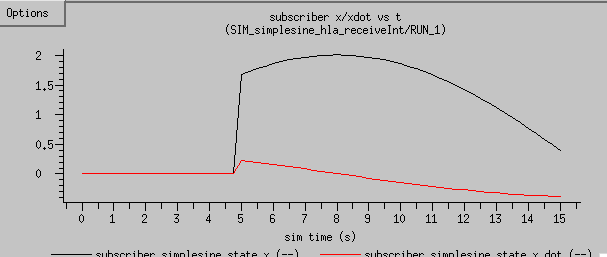
\includegraphics[width=4.5in]{TrickHLAUser-receiveInt.png}
  \end{center}
\caption{$x(t)$ and $\dot{x}(t)$ from {\tt SIM\_simplesine\_hla\_receiveInt}}
\label{fig:hla-receiveInt}
\end{figure}
